
The previous experiments were conducted in a non-linear structured setting where we are unaware of a provably near-optimal algorithm.
% 
To assess how close \pred's regret is to optimal, in this section, we consider a \textit{linear} setting for which there exist well-understood algorithms \citep{abbasi2011improved,lattimore2020bandit}.
% In this section, we show the performance of \pred\ when the reward structure per task is linear and try to understand the exploration of \pred. Note that we evaluate \pred\ in the linear bandit setting as it is well understood theoretically and empirically optimal algorithms exist for this setting \citep{abbasi2011improved, lattimore2020bandit}.
% 
Such algorithms provide a strong upper bound for \pred. We summarize the key finding below:

\begin{tcolorbox}
\customfinding \pred\ (\gt) matches the performance of the optimal algorithm \linucb\ in linear bandit setting as it learns to exploit the latent structure across tasks from in-context data and without access to features.
% It learns to exploit the latent structure of the underlying tasks even when it is trained without the optimal action $a_{m,*}$ (or its approximation) and without the action features $\X$.
\end{tcolorbox}

In \Cref{fig:short-horizon-lin} we first show the linear bandit setting for horizon $n=25$, $\Mpr = 200000$, $\Mts = 200$, $A=10$, and $d=2$. 
%
%
Note that the length of the context (the number of rounds) is an artifact of the transformer architecture and computational complexity. This is because the self-attention takes in as input a length-$n$ sequence of tokens of size $d$, and requires $O\left(d n^2\right)$ time to compute the output \citep{keles2023computational}. 
%
Further empirical setting details are stated in \Cref{sec:addl-expt}.
%

We observe from \Cref{fig:short-horizon-lin}  that \pred\ (\gt) has lower cumulative regret than \dptg, and \ad. Note that for this low data (short horizon) regime, the \dptg\ does not have a good estimation of $\widehat{a}_{m,*}$ which results in a poor prediction of optimal action $\widehat{a}_{m,t,*}$. This results in higher regret. Observe that \pred\ (\gt) performs quite similarly to \linucb\ and lowers regret compared to \ts\ which also shows that \pred\ is able to exploit the latent linear structure and reward correlation of the underlying tasks.
%
Note that \linucb\ is close to the optimal algorithm for this linear bandit setting. 
% \smnote{Should we say this line? LinTS is known to perform better than \linucb}. 
%
\pred\ outperforms \ad\ as the main objective of \ad\ is to match the performance of its demonstrator.
% \ad\ is not able to outperform its demonstrator \ts\ as it is trained to predict the next action of the demonstrator. 
In this short horizon, we see that \mlin\ performs similarly to \linucb. 

We also show how the prediction error of the optimal action by \pred\ is small compared to \linucb\ in the linear bandit setting. In \Cref{fig:lin-action-dist} we first show how the $10$ actions are distributed in the $\Mts=200$ test tasks. In \Cref{fig:lin-action-dist} for each bar, the frequency indicates the number of tasks where the action (shown in the x-axis) is the optimal action. Then, in \Cref{fig:lin-action-error}, we show the prediction error of \pred\ (\gt) for each task $m\in[\Mts]$. The prediction error is calculated as $(\wmu_{m,n, *}(a) - \mu_{m, *}(a))^2$ where $\wmu_{m,n, *}(a) = \max_a\wtheta_{m,n}^\top\bx_m(a)$ is the empirical mean at the end of round $n$, and $\mu_{*,m}(a)=\max_a\btheta_{m,*}^\top\bx_m(a)$ is the true mean of the optimal action in task $m$. Then we average the prediction error for the action $a\in [A]$ by the number of times the action $a$ is the optimal action in some task $m$. 
%
From the \Cref{fig:lin-action-error}, we see that for actions $\{2,3,5,6,7,10\}$, the prediction error of \pred\ is either close or smaller than \linucb. 
% This constitutes nearly $70\%$ of the $200$ test tasks. 
Note that \linucb\ estimates the empirical mean directly from the test task, whereas \pred\ has a strong prior based on the training data. So \pred\ is able to estimate the reward of the optimal action quite well from the training dataset $\Dpr$.
%
This shows the power of \pred\ to go beyond the in-context decision-making setting studied in \citet{lee2023supervised, lin2023transformers, ma2023rethinking, sinii2023context, liu2023reason} which require long horizons/trajectories and optimal action during training to learn a near-optimal policy. 

% We discuss how exploration of \pred\ (\gt) results in low cumulative regret in \Cref{sec:exploration}. 
%
% Importantly, we show that predicting the reward has significant advantages in a low-data regime as it leads to the right notion of exploration.


% \begin{figure}[!hbt]
% \centering
% \vspace*{-1em}
% \begin{tabular}{ccc}
% \subfigure[Linear Bandit setting]{\hspace*{-1.5em}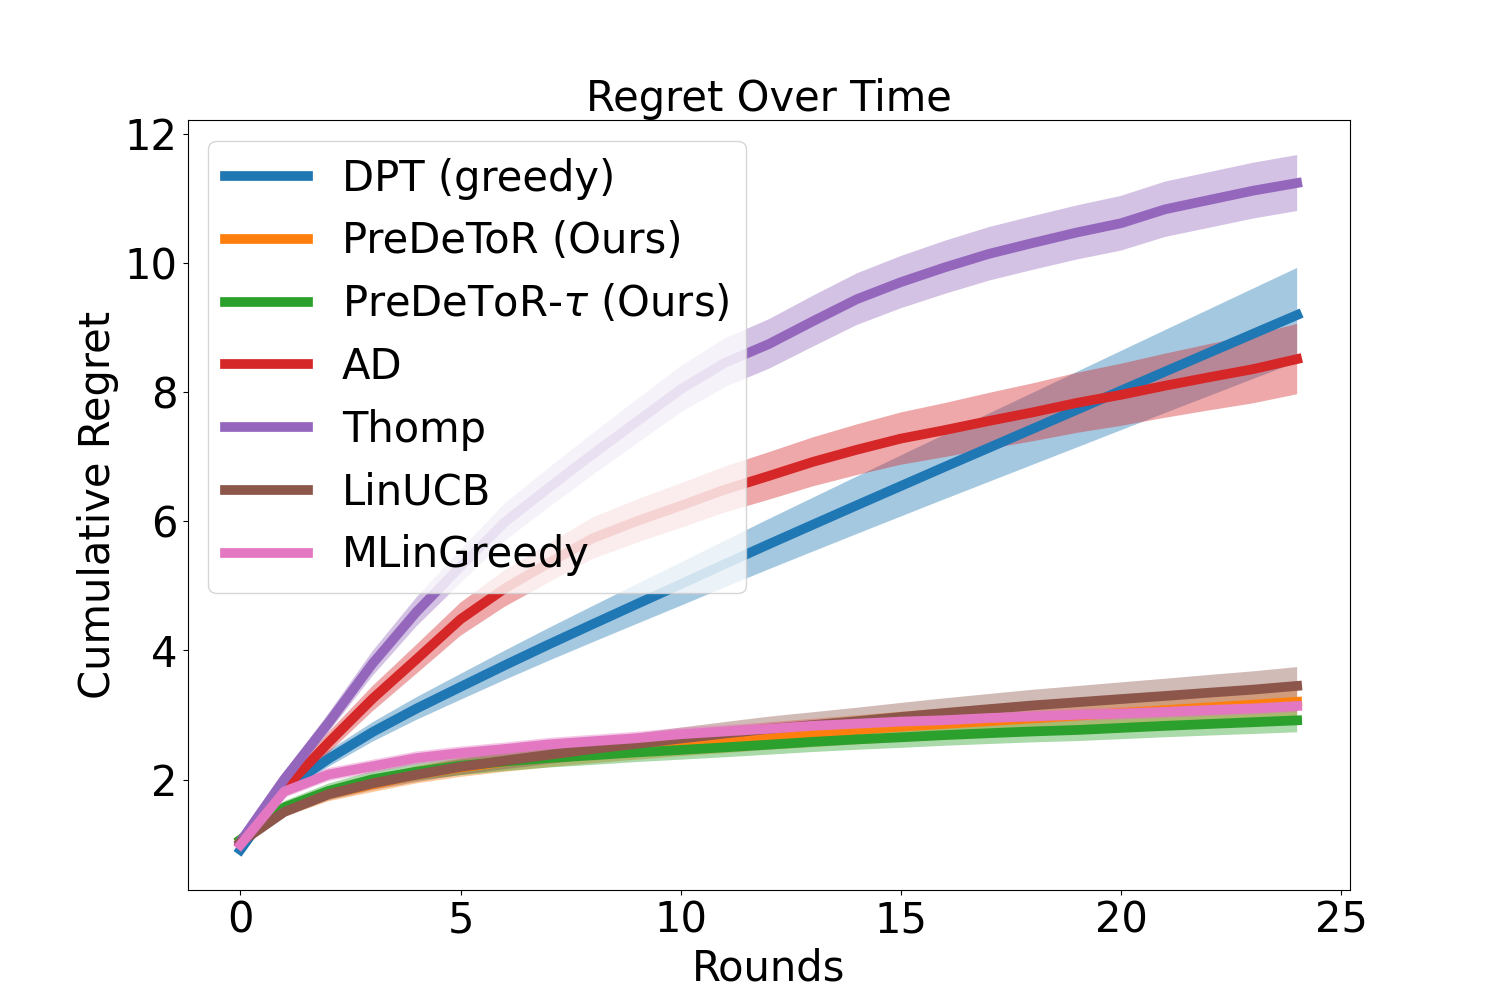
\includegraphics[scale = 0.1]{img/Neurips/linear/lin_lr0.00015_do0_embd32_layer4_head4_envs100000_hists1_samples1_var0.3_cov0.0_H25_d10_lind2_seed1_testcov0.0_hor25.pkl.png} \label{fig:lin}} &
% %%%%%%%%%%
% % \hspace*{-1.5em}\subfigure[Non-linear bandit]{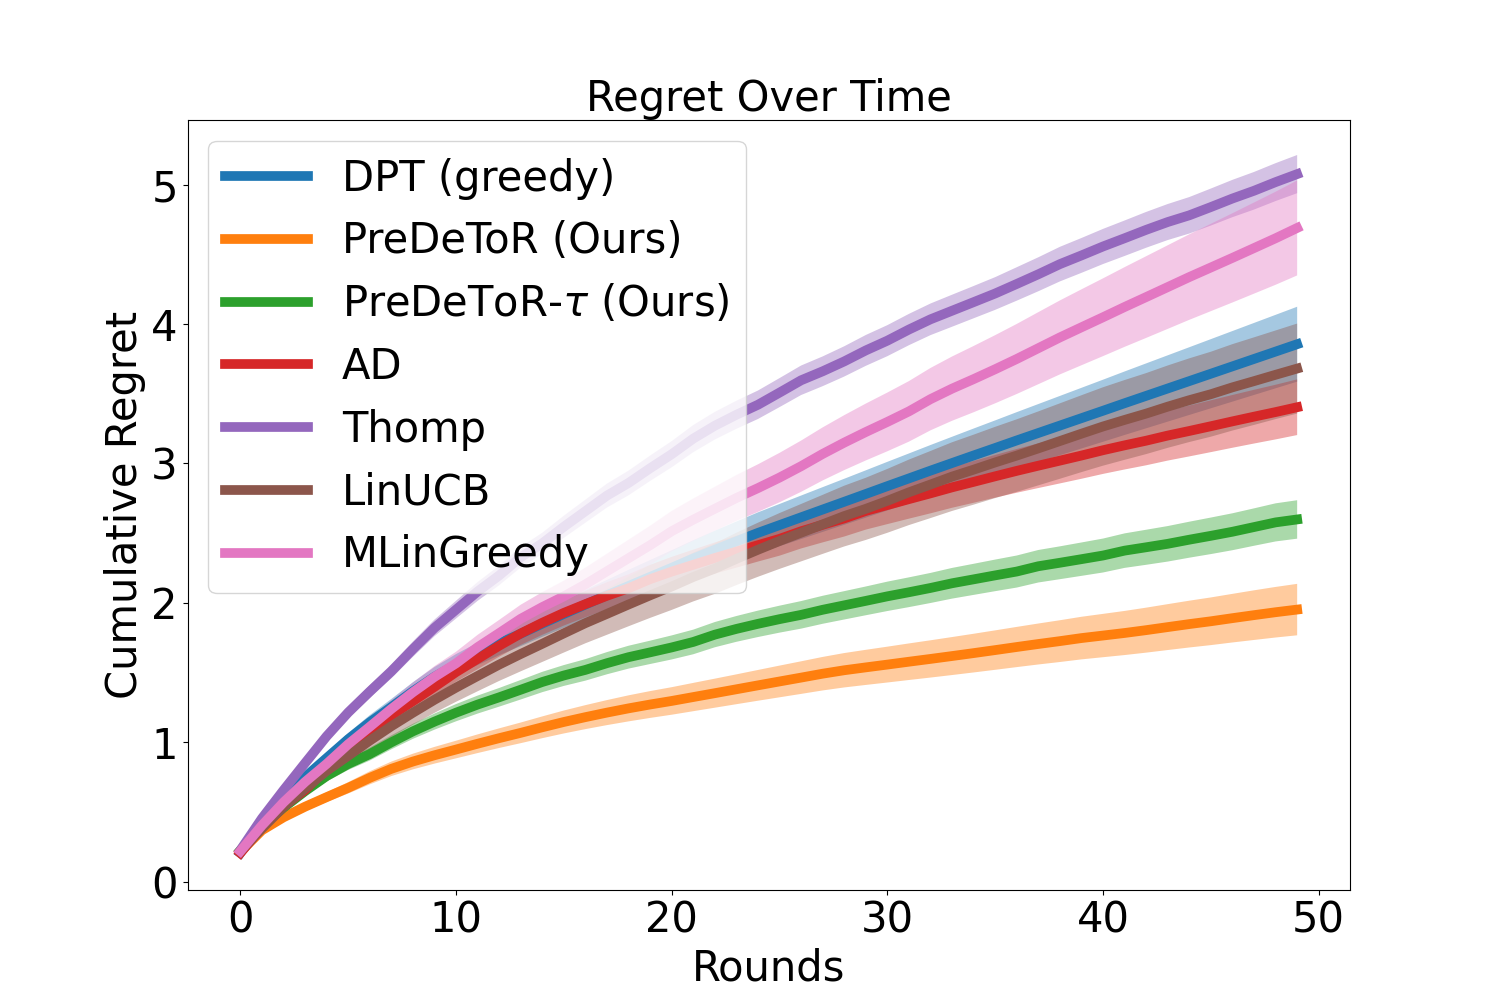
\includegraphics[scale = 0.1]{img/Neurips/non_linear/nlm_lr0.00015_do0_embd32_layer4_head4_envs100001_hists1_samples1_var0.3_cov0.0_H50_d6_lind2_seed1_testcov0.0_hor50.pkl.png} \label{fig:short-horizon-nlm}} &%\\
% %%%%%%%%%%%%%%%%%%%%%%%
% \hspace*{-1.5em}\subfigure[Test action distribution]{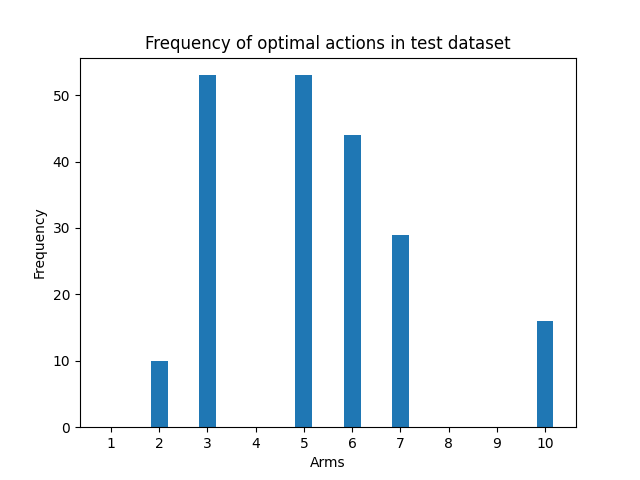
\includegraphics[scale = 0.21]{img/Neurips/linear/optimal_action_test.png} \label{fig:lin-action-dist}}&
% % %%%%%%%%%%
% \hspace*{-1.5em}\subfigure[Test Prediction Error]{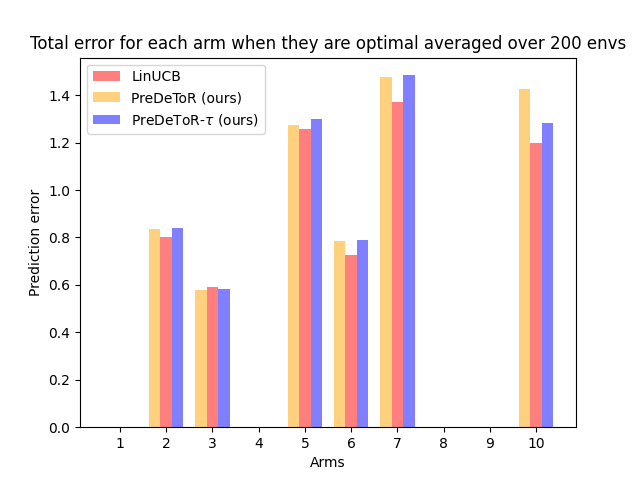
\includegraphics[scale = 0.21]{img/Neurips/linear/analysis_total.png} \label{fig:lin-action-error}}
% \end{tabular}
% \vspace*{-1em}
% \caption{Linear Expt. The horizontal axis is the number of rounds. Confidence bars show one standard error.}
% \label{fig:short-horizon-lin}
% \vspace{-0.7em}
% \end{figure}


\begin{figure}[!hbt]
\centering
\vspace*{-1em}
\begin{subfigure}[b]{0.32\textwidth}
    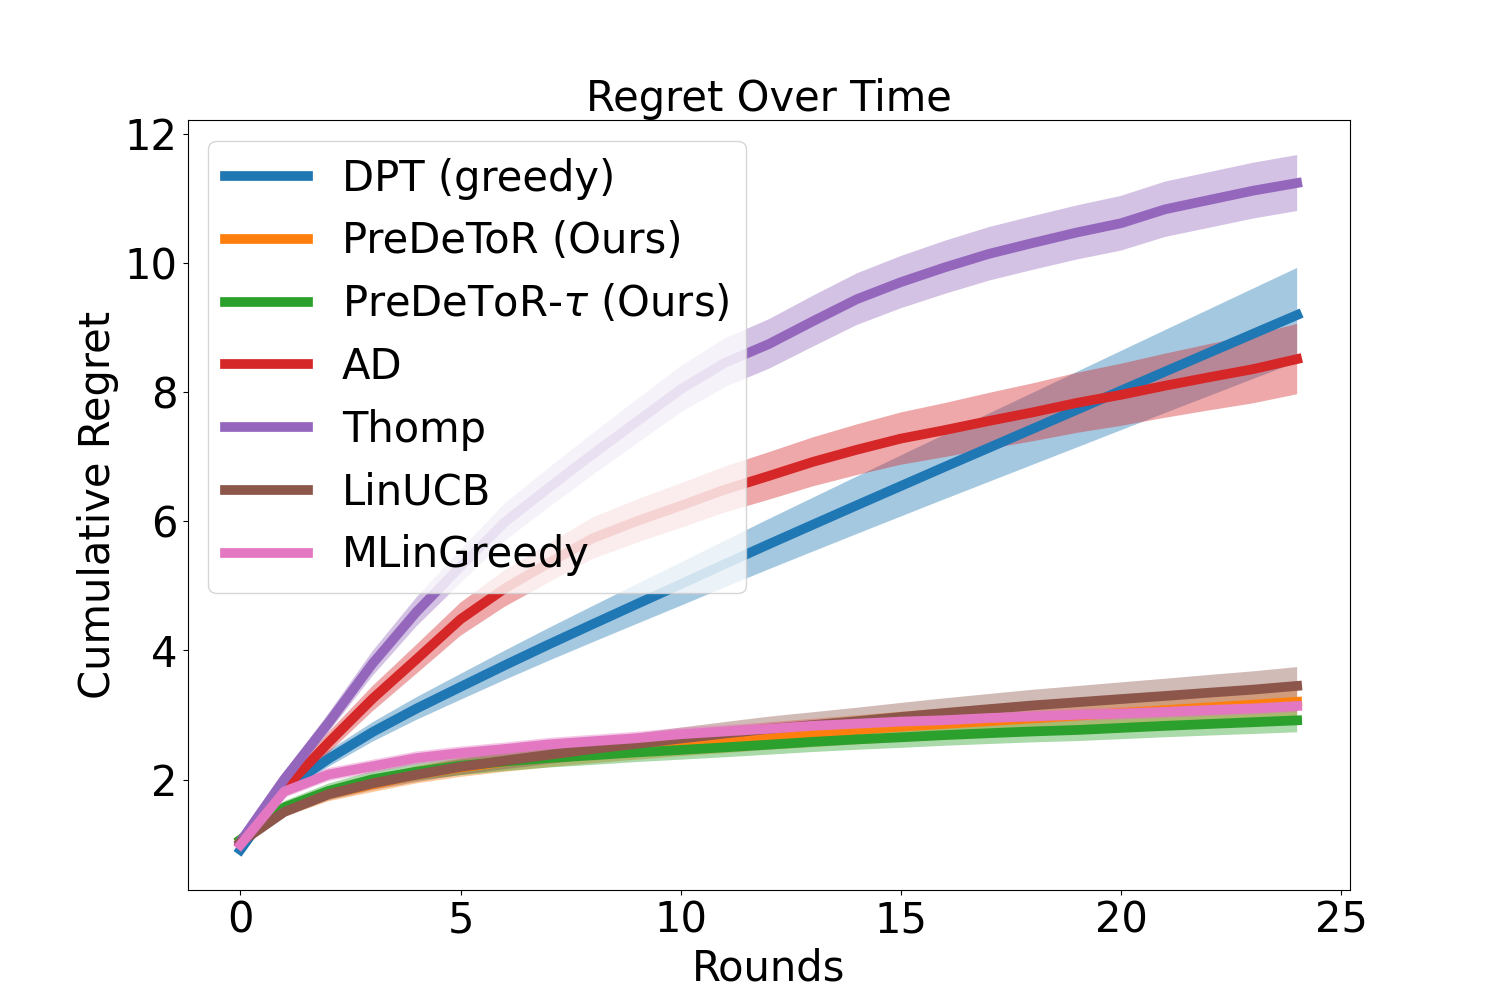
\includegraphics[scale=0.1]{img/Neurips/linear/lin_lr0.00015_do0_embd32_layer4_head4_envs100000_hists1_samples1_var0.3_cov0.0_H25_d10_lind2_seed1_testcov0.0_hor25.pkl.png}
    \caption{Linear Bandit setting}
    \label{fig:lin}
\end{subfigure}%
% Comment out for reference
% \begin{subfigure}[b]{0.32\textwidth}
%     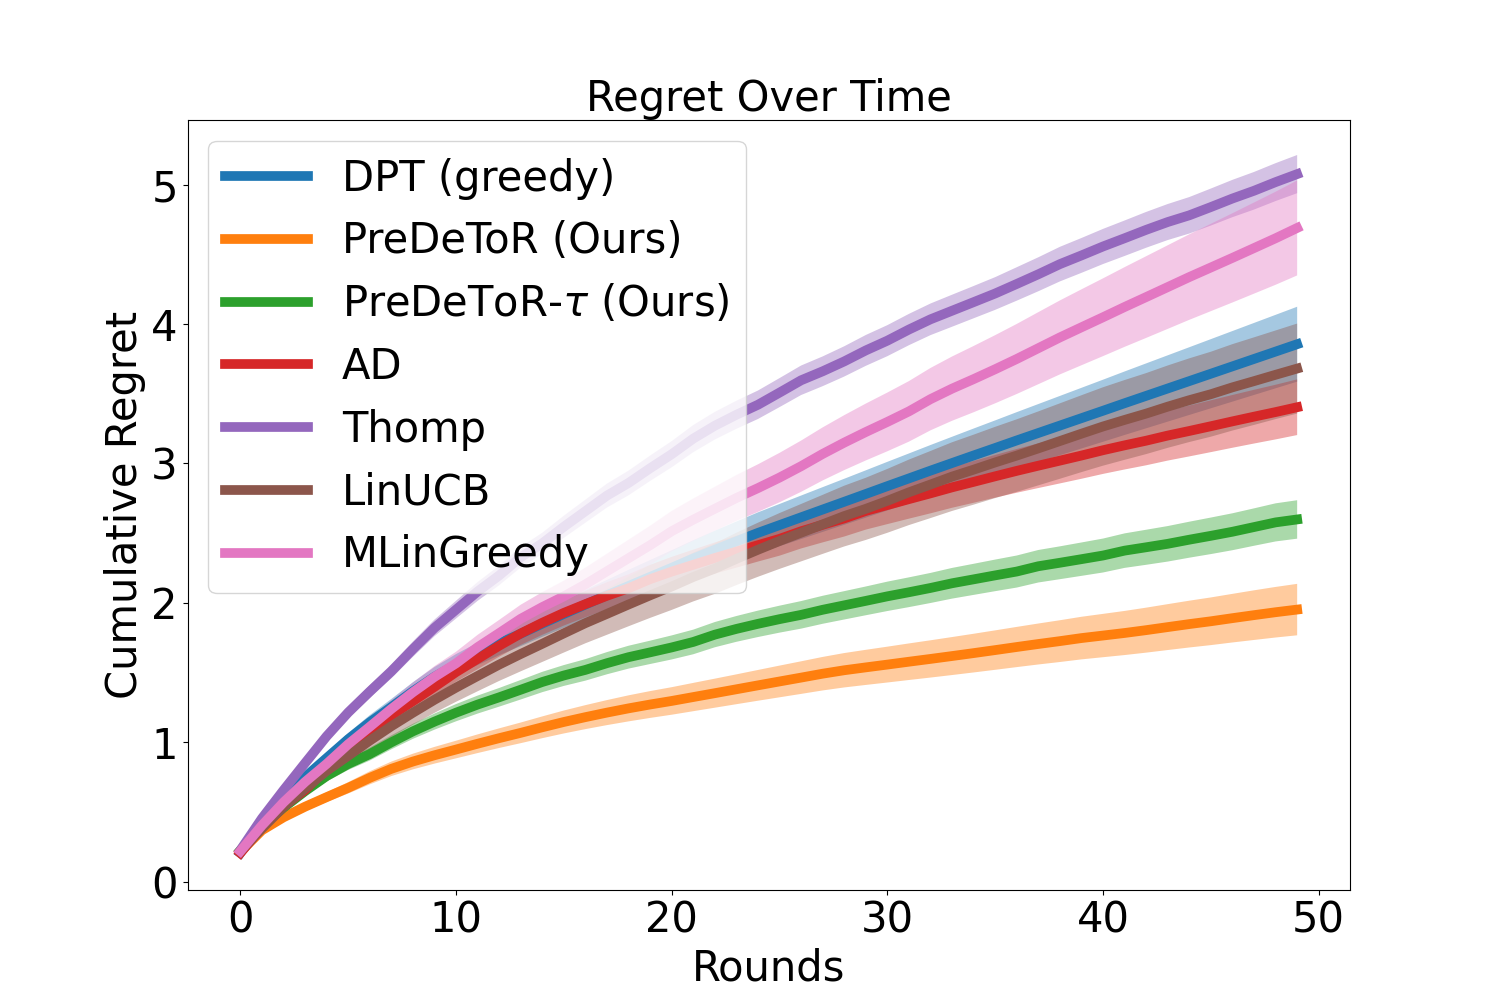
\includegraphics[scale=0.1]{img/Neurips/non_linear/nlm_lr0.00015_do0_embd32_layer4_head4_envs100001_hists1_samples1_var0.3_cov0.0_H50_d6_lind2_seed1_testcov0.0_hor50.pkl.png}
%     \caption{Non-linear bandit}
%     \label{fig:short-horizon-nlm}
% \end{subfigure}%
\begin{subfigure}[b]{0.32\textwidth}
    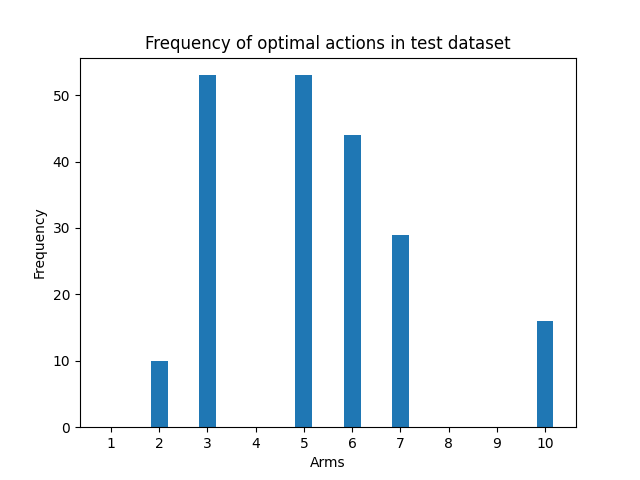
\includegraphics[scale=0.21]{img/Neurips/linear/optimal_action_test.png}
    \caption{Test action distribution}
    \label{fig:lin-action-dist}
\end{subfigure}%
\begin{subfigure}[b]{0.32\textwidth}
    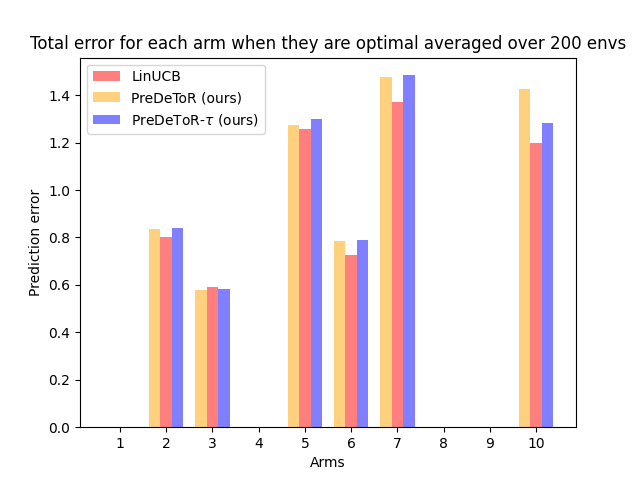
\includegraphics[scale=0.21]{img/Neurips/linear/analysis_total.png}
    \caption{Test Prediction Error}
    \label{fig:lin-action-error}
\end{subfigure}
\vspace*{-1em}
\caption{Linear Expt. The horizontal axis is the number of rounds. Confidence bars show one standard error.}
\label{fig:short-horizon-lin}
\vspace{-0.7em}
\end{figure}

% \subsection{Exploration of \pred (\gt)}
% \label{sec:exploration}
% In this section, we discuss the exploration of \pred\ in the linear bandit setting discussed in \Cref{sec:short-horizon}. Recall that the linear bandit setting consist of horizon $n=25$, $\Mpr = 200000$, $\Mts = 200$, $A=10$, and $d=2$. 
% %
% %
% The demonstrator $\pi^w$ is the \ts\ algorithm and we observe that \pred\ (\gt) has lower cumulative regret than \dptg, \ad\ and matches the performance of \linucb. 
% % 
% Therefore \pred\ (\gt) behaves almost optimally in this setting and so we analyze how \pred\ conducts exploration for this setting.  
% %



% \textbf{Outcomes:} We first discuss the main outcomes of our analysis of exploration in the low-data regime:

We now state the main finding of our analysis of exploration in the linear bandit setting:

\begin{tcolorbox}
\customfinding The \pred\ (\gt) has an implicit two-phase exploration. In the first phase, it explores with a strong prior over the in-context training data. In the second phase, once the task data has been observed for a few rounds (in-context) it switches to task-based exploration.
\end{tcolorbox}

% \noindent
% \textbf{(1)} The \pred\ (\gt) has a two phase exploration. In the first phase it explores with a strong prior over the training data. In the second phase, once the task data has been observed for a few rounds it switches to task-based exploration.

% \textbf{(2)} \pred\ (\gt) samples the optimal action in each task more than \dptg. \pred (\gt) considers a larger set of possible optimal action candidate set than \dptg.




We first show in \Cref{fig:train-dist} the training distribution of the optimal actions. For each bar, the frequency indicates the number of tasks where the action (shown in the x-axis) is the optimal action.
%
Then in \Cref{fig:analysis-epxploration} we show how the sampling distribution of \dptg, \pred\, and \predt\ change in the first $10$ and last $10$ rounds for all the tasks where action $5$ is optimal. To plot this graph we first sum over the individual pulls of the action taken by each algorithm over the first $10$ and last $10$ rounds. Then we average these counts over all test tasks where action $5$ is optimal. From the figure \Cref{fig:analysis-epxploration} we see that \pred (\gt) consistently pulls the action $5$ more than \dptg. It also explores other optimal actions like $\{2,3,6,7,10\}$ but discards them quickly in favor of the optimal action $5$ in these tasks. This shows that \pred\ (\gt) only considers the optimal actions seen from the training data. Once sufficient observation have been observed for the task it switches to task-based exploration and samples the optimal action more than \dptg.

Finally, we plot the feasible action set considered by \dptg, \pred, and \predt\ in \Cref{fig:analysis-exploration-time}. To plot this graph again we consider the test tasks where the optimal action is $5$. Then we count the number of distinct actions that are taken from round $t$ up until horizon $n$. Finally we average this over all the considered tasks where the optimal action is $5$. We call this the candidate action set considered by the algorithm. From the \Cref{fig:analysis-exploration-time} we see that \dptg\ explores the least and gets stuck with few actions quickly (by round $10$). Note that the actions \dptg\ samples are sub-optimal and so it suffers a high cumulative regret (see \Cref{fig:short-horizon-lin}).  \pred\ explore slightly more than \dptg, but \predt\ explores the most. 
%
% \begin{figure}[!hbt]
% \centering
% \begin{tabular}{ccc}
% \subfigure[Train Optimal Action Distribution]{\hspace*{-0.7em}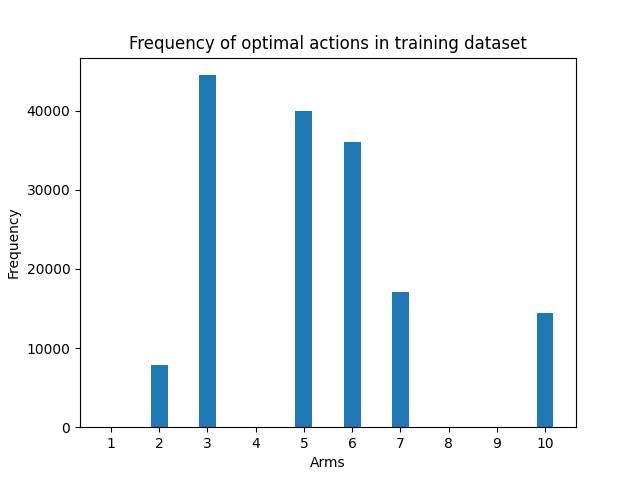
\includegraphics[scale = 0.27]{img/Neurips/linear/optimal_action_train.png}\label{fig:train-dist}} &
% %%%%%%%%%%
% \hspace*{-0.7em}\subfigure[Distribution of action sampling in all tasks where action $5$ is optimal]{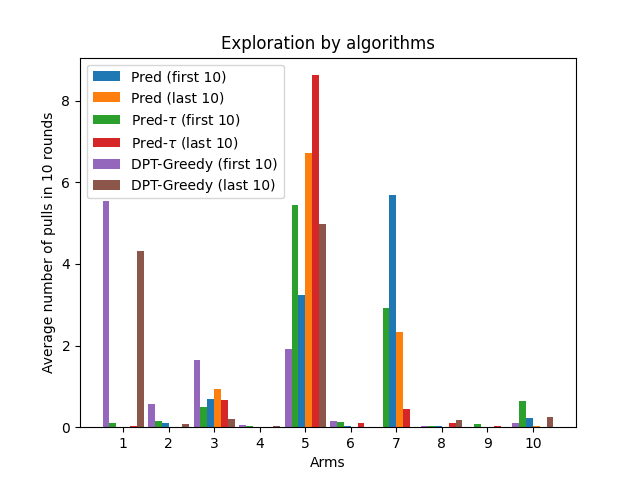
\includegraphics[scale = 0.27]{img/Neurips/linear/analysis_pull.png} \label{fig:analysis-epxploration}} &
% %%%%%%%%%%%%%%%%%%%%%%%
% \subfigure[Candidate Action Set in Time averaged over all tasks where action $5$ is optimal]{\hspace*{-0.7em}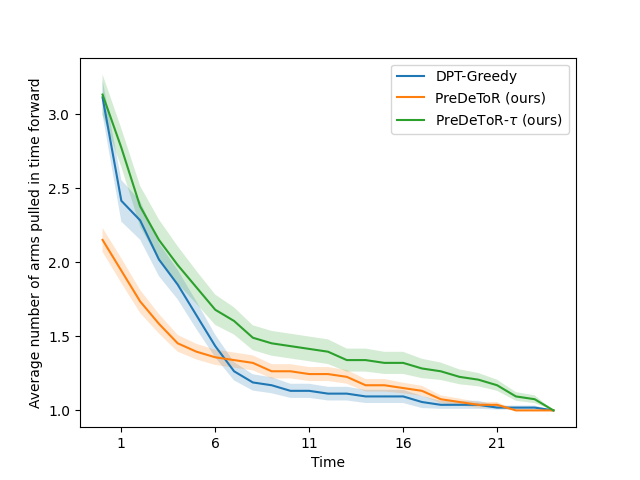
\includegraphics[scale = 0.27]{img/Neurips/linear/analysis_time_1.png}\label{fig:analysis-exploration-time}} 
% \end{tabular}
% \caption{Exploration Analysis of \pred (\gt)}
% \label{fig:exploration-analysis-time}
% \end{figure}
%
\begin{figure}[!hbt]
\vspace*{-1em}
\centering
\begin{subfigure}[b]{0.27\textwidth}
   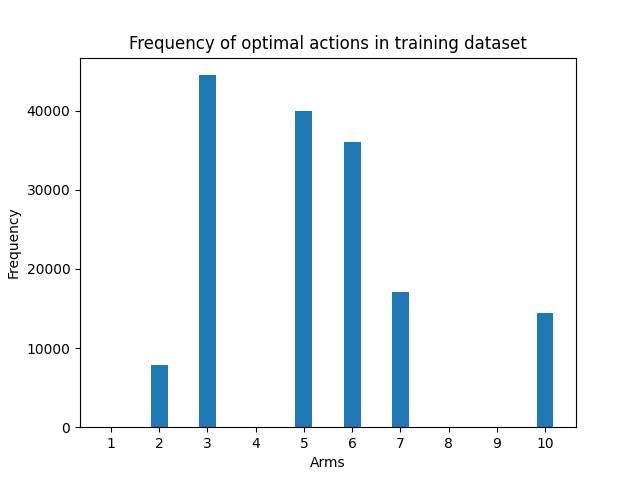
\includegraphics[scale=0.25]{img/Neurips/linear/optimal_action_train.png}
   \caption{Train Optimal Action Distribution}
   \label{fig:train-dist}
\end{subfigure}%
\hspace*{1em}\begin{subfigure}[b]{0.27\textwidth}
   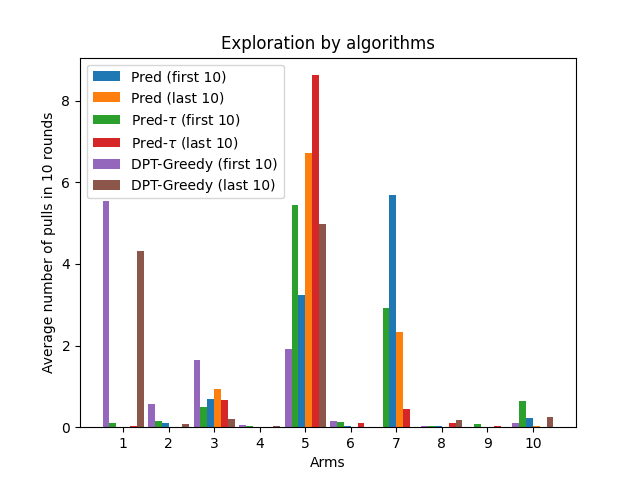
\includegraphics[scale=0.25]{img/Neurips/linear/analysis_pull.png}
   \caption{Distribution of action sampling in all test tasks where action $5$ is optimal}
   \label{fig:analysis-epxploration}
\end{subfigure}%
\hspace*{1em}\begin{subfigure}[b]{0.27\textwidth}
   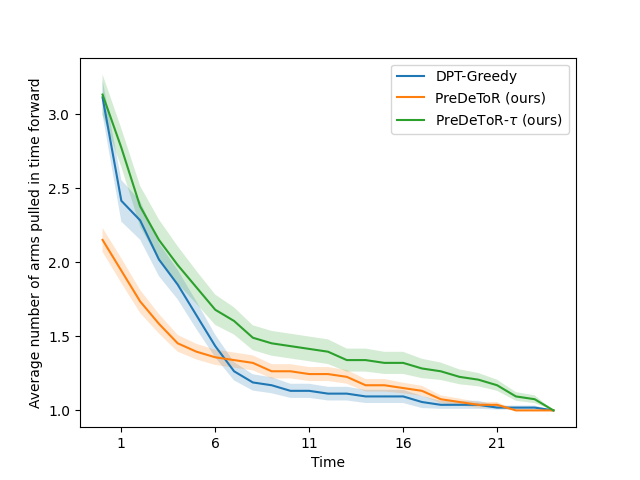
\includegraphics[scale=0.25]{img/Neurips/linear/analysis_time_1.png}
   \caption{Candidate Action Set in Time averaged over all tasks where action $5$ is optimal}
   \label{fig:analysis-exploration-time}
\end{subfigure}
\caption{Exploration Analysis of \pred (\gt)}
\label{fig:exploration-analysis-time}
\end{figure}
\vspace*{-1em}